\subsubsection{Iteration}

\YIComment{Redo this}

\autoref{figure:primal-mips} shows the performance of the \texttt{primal(n)} test suite. It can be seen that as \texttt{n} increases, the performance increases rapidly on both SUTs.

The interpreter has higher initial performance but stabilizes at a lower peak performance and at a lower value of \texttt{n}. This is because the interpreter doesn't speedup much from executing the same blocks repeatedly as there is no caching or reuse involved. It does however still see a large improvement when \texttt{n} is low because at this range the fixed overheads and initialization costs are still relatively high, and hence executing more source instructions amortizes those costs. Furthermore, repeated execution of the same instructions allow the branch predictor to become more accurate and the instruction cache warmer, both contributing to increased performance.

The JIT emulator on the other hand sees a far higher peak performance, but much worse initial performance and takes longer to achieve high performance. This is because, in addition to the higher overhead costs for the JIT emulator, each block of source code also has a high associated compilation costs. As \texttt{n} increases the same blocks are executed many times, amortizing the fixed compilation costs. This allows the JIT emulator to achieve a very high performance due to its far superior execution performance.

\begin{figure}[h]
    \centering
    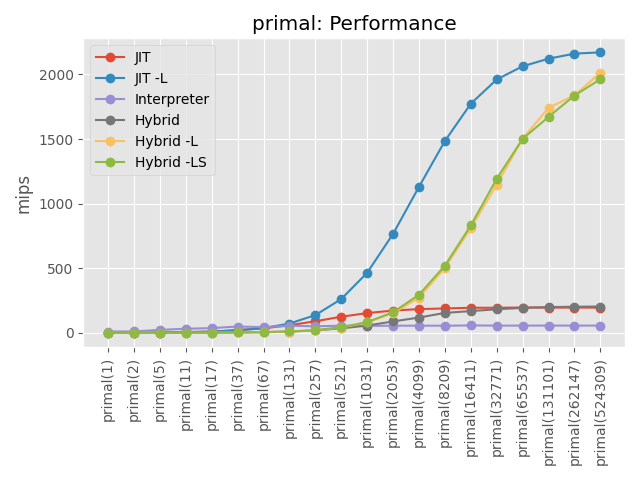
\includegraphics[scale=0.75]{output/graphs/tests/all/primal/mips.png}
    \caption{Performance in mips of the primal test suite.}
    \label{figure:primal-mips}
\end{figure}